\section{Background Correction}

Effects which involve particles being undetected are group together under efficiency effects. There are many reasons why this can occur such as from particles which travel along the beam pipe of an accelerator bypassing the sensitive instruments of the detector; particles which leave weak signals in sensitive components; have low momentum and are swept out of the detector; neutral particles which interact weakly etc. The result of these effects are to decrease the ratio of number of detected particles to the number of generated particles. Conversely effects which produce false, duplicate copies or detector induced particles are grouped together as false or background particles. This may occur when hits from several particles incorrectly associated together; hits from a particle are not all associated together but instead form subgroups; particles interact with material in the detector to cause showers of particles. In order to understand the underlying physics of the initial interaction these effects must be disentangled, this process is known as unfolding.

The first stage of the unfolding procedure is to remove the background contribution from the kinematic track distributions and track multiplicity distributions. Background tracks are classified as follows,

\begin{table}[htdp]
	\caption{Background track classifications}
		\begin{center}
			\begin{tabular}{|c|p{0.7\textwidth}|}
				\hline
				Ghost track & Tracks which are either a) not associated to any corresponding true particle either from the initial proton-proton interaction or from their interactions with detector material and magnetic fields b) has only a small fraction of hits associated from a true particle.  \\
				\hline
				 Material track & Tracks which are a result of the interaction between particles from the initial proton-proton reaction and detector material. In MC simulated data material tracks are determined by tracks which are associated to particles that are not involved in the generator level event description \\
				 \hline
				 Secondary track & Tracks associated to true particles which do not meet the prompt particle requirement \\
				 \hline
				 Clone track & Tracks associated to true prompt particles and share the same association with other tracks in the event \\
				\hline
			\end{tabular}
		\end{center}
	\label{default}
\end{table}%

To correct for background contributions the mean purity, $p$, is calculated for $\eta$, $p_T$, $n_{velo}$, $n_{t}$ bins, where $n_{velo}$ is the number of Velo tracks reconstructed in the event and $n_t$ is the number of hits in the T-stations for the event.

\begin{equation}
	p(\eta, p_T, n_{velo}, n_t) = \frac{n_{mat}(\eta, p_T, n_{velo}, n_t)}{n_{reco}(\eta, p_T, n_{velo}, n_t)}
\end{equation}

\begin{figure}
	\begin{subfigure}[h]{0.49\textwidth}
		\includegraphics[width=\textwidth]{/afs/cern.ch/work/d/dvoong/private/cmtuser/DaVinci_v33r6/Phys/ChargedParticleMultiplicity/python/efficiency_and_purity/data_files/bk/Down/mc/-1/-1/bk/Down/mc/-1/-1/meissner/pngs/purity/signal.png}
		\caption{Signal weight}
		\label{fig: signal weight}
	\end{subfigure}
	\begin{subfigure}[h]{0.49\textwidth}
		\includegraphics[width=\textwidth]{/afs/cern.ch/work/d/dvoong/private/cmtuser/DaVinci_v33r6/Phys/ChargedParticleMultiplicity/python/efficiency_and_purity/data_files/bk/Down/mc/-1/-1/bk/Down/mc/-1/-1/meissner/pngs/purity/signal_matched.png}
		\caption{Signal Matched weight}
		\label{fig: signal matched weight}
	\end{subfigure}
	\caption{Signal weights as a function of $\eta$ and $\mathrm{p}_T$.}
	\label{fig: signal weights}
\end{figure}

\begin{figure}
	\centering
	\begin{subfigure}[h]{0.49\textwidth}
		\includegraphics[width=\textwidth]{/afs/cern.ch/work/d/dvoong/private/cmtuser/DaVinci_v33r6/Phys/ChargedParticleMultiplicity/python/efficiency_and_purity/data_files/bk/Down/mc/-1/-1/bk/Down/mc/-1/-1/meissner/pngs/purity/ghost.png}
		\caption{Ghost Rate}
		\label{}
	\end{subfigure}
	\begin{subfigure}[h]{0.49\textwidth}
		\includegraphics[width=\textwidth]{/afs/cern.ch/work/d/dvoong/private/cmtuser/DaVinci_v33r6/Phys/ChargedParticleMultiplicity/python/efficiency_and_purity/data_files/bk/Down/mc/-1/-1/bk/Down/mc/-1/-1/meissner/pngs/purity/outside_bin.png}
		\caption{Bin Migration Rate}
		\label{}
	\end{subfigure}
	\begin{subfigure}[h]{0.49\textwidth}
		\includegraphics[width=\textwidth]{/afs/cern.ch/work/d/dvoong/private/cmtuser/DaVinci_v33r6/Phys/ChargedParticleMultiplicity/python/efficiency_and_purity/data_files/bk/Down/mc/-1/-1/bk/Down/mc/-1/-1/meissner/pngs/purity/secondary.png}
		\caption{Secondary Rate}
		\label{}
	\end{subfigure}
	\begin{subfigure}[h]{0.49\textwidth}
		\includegraphics[width=\textwidth]{/afs/cern.ch/work/d/dvoong/private/cmtuser/DaVinci_v33r6/Phys/ChargedParticleMultiplicity/python/efficiency_and_purity/data_files/bk/Down/mc/-1/-1/bk/Down/mc/-1/-1/meissner/pngs/purity/material.png}
		\caption{Material Rate}
		\label{}
	\end{subfigure}
	\begin{subfigure}[h]{0.49\textwidth}
		\includegraphics[width=\textwidth]{/afs/cern.ch/work/d/dvoong/private/cmtuser/DaVinci_v33r6/Phys/ChargedParticleMultiplicity/python/efficiency_and_purity/data_files/bk/Down/mc/-1/-1/bk/Down/mc/-1/-1/meissner/pngs/purity/clone.png}
		\caption{Clone Rate}
		\label{}
	\end{subfigure}
	\caption{Background Rates}
	\label{fig: background rates}
\end{figure}

where $n_{mat}$ is the number of tracks matched to a prompt particle in the same $\eta$, $p_T$ and $n_{velo}$ bin. The background corrected $\eta$ and $p_T$ distributions are calculated by weighting each track by its corresponding purity. 

\begin{figure}[h]
	\begin{subfigure}{0.49\textwidth}
		\includegraphics[width=\textwidth]{/afs/cern.ch/user/d/dvoong/cmtuser/DaVinci_v33r6/Phys/ChargedParticleMultiplicity/python/kinematic_distributions/tracks/data_files/plots/bk/Down/mc/-1/-1/bk/Down/mc/-1/-1/meissner/bk/Down/real/-1/-1/bk/Down/real/-1/-1/pngs/track_distributions/background_corrected/eta_norm.png}
		\caption{$\eta$}
		\label{fig: background corrected track distributions eta}
	\end{subfigure}
%	\begin{subfigure}[h]{0.49\textwidth}
%		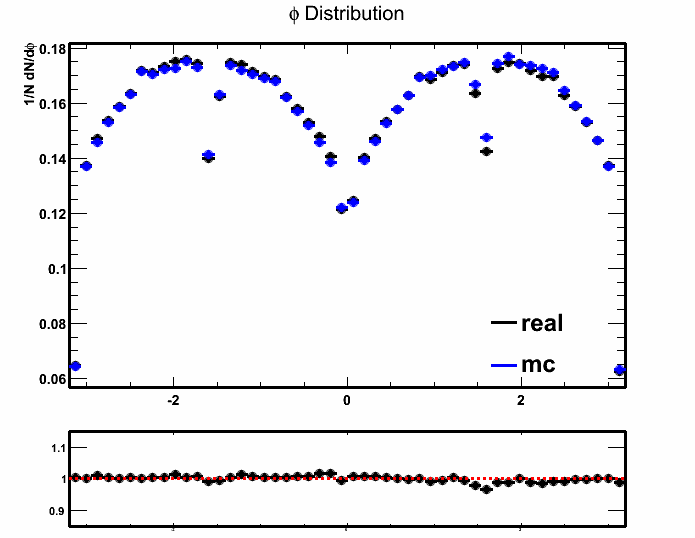
\includegraphics[width=\textwidth]{./Chapters/multiplicity/images/phi_background_corrected.png}
%		\caption{$\phi$}
%		\label{fig: background corrected track distributions phi}
%	\end{subfigure}
	\begin{subfigure}[h]{0.49\textwidth}
		\includegraphics[width=\textwidth]{/afs/cern.ch/user/d/dvoong/cmtuser/DaVinci_v33r6/Phys/ChargedParticleMultiplicity/python/kinematic_distributions/tracks/data_files/plots/bk/Down/mc/-1/-1/bk/Down/mc/-1/-1/meissner/bk/Down/real/-1/-1/bk/Down/real/-1/-1/pngs/track_distributions/background_corrected/pt_norm.png}
		\caption{$p_T$}
		\label{fig: background corrected track distributions pt}
	\end{subfigure}
%	\begin{subfigure}[h]{0.49\textwidth}
%		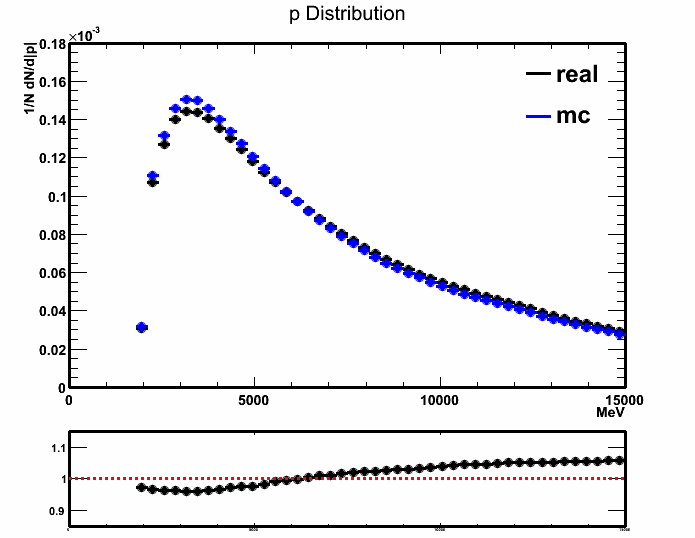
\includegraphics[width=\textwidth]{./Chapters/multiplicity/images/p_background_corrected.png}
%		\caption{$|p|$}
%		\label{fig: background corrected track distributions p}
%	\end{subfigure}
	\caption{Background corrected track distributions}
	\label{fig: background corrected track distributions}
\end{figure}

\begin{figure}[h]
	\begin{subfigure}{0.49\textwidth}
		\includegraphics[width=\textwidth]{/afs/cern.ch/user/d/dvoong/cmtuser/DaVinci_v33r6/Phys/ChargedParticleMultiplicity/python/kinematic_distributions/tracks/data_files/plots/bk/Down/mc/-1/-1/bk/Down/mc/-1/-1/meissner/bk/Down/real/-1/-1/bk/Down/real/-1/-1/pngs/comparison/background_corrected/eta_comparison_norm.png}
		\caption{$\eta$}
		\label{fig: background corrected track distributions eta}
	\end{subfigure}
	\begin{subfigure}{0.49\textwidth}
		\includegraphics[width=\textwidth]{/afs/cern.ch/user/d/dvoong/cmtuser/DaVinci_v33r6/Phys/ChargedParticleMultiplicity/python/kinematic_distributions/tracks/data_files/plots/bk/Down/mc/-1/-1/bk/Down/mc/-1/-1/meissner/bk/Down/real/-1/-1/bk/Down/real/-1/-1/pngs/comparison/background_corrected/pt_comparison_norm.png}
		\caption{$p_T$}
		\label{fig: background corrected track distributions pt}
	\end{subfigure}
	\caption{Background corrected track distributions, MC and measured data comparison}
	\label{fig: background corrected track distributions, MC and measured data comparison}
\end{figure}

\begin{figure}[h]
	\begin{subfigure}{0.49\textwidth}
		\includegraphics[width=\textwidth]{/afs/cern.ch/user/d/dvoong/cmtuser/DaVinci_v33r6/Phys/ChargedParticleMultiplicity/python/kinematic_distributions/tracks/data_files/plots/bk/Down/mc/-1/-1/bk/Down/mc/-1/-1/meissner/bk/Down/mc/-1/-1/bk/Down/mc/-1/-1/pngs/cross_check/eta_background_correction_cross_check.png}
		\caption{$\eta$}
	\end{subfigure}
	\begin{subfigure}{0.49\textwidth}
		\includegraphics[width=\textwidth]{/afs/cern.ch/user/d/dvoong/cmtuser/DaVinci_v33r6/Phys/ChargedParticleMultiplicity/python/kinematic_distributions/tracks/data_files/plots/bk/Down/mc/-1/-1/bk/Down/mc/-1/-1/meissner/bk/Down/mc/-1/-1/bk/Down/mc/-1/-1/pngs/cross_check/pt_background_correction_cross_check.png}
		\caption{$p_T$}
	\end{subfigure}
	\caption{Background correction cross-check. Background corrected track distributions are compared with tracks matched to generator prompt particles by MC truth matching}
	\label{fig: background correction cross-check}
\end{figure}

To correct for the background contribution to track multiplicity this same method cannot be used since it would result in non-integer multiplicities. Instead the background is modelled with a Poisson distribution,

\begin{equation*}
	f(k; \lambda) = \frac{\lambda^{k}e^{-\lambda}}{k!}
\end{equation*}

where $k$ corresponds to the number of background tracks in an event and $\lambda$ corresponds to the expected number of background tracks calculated by summing the background rates for all tracks in the event,

\begin{equation}
	\lambda = \sum^{N}_{i=0} 1 - p_i(\eta, p_T, n_{velo}, n_t)
\end{equation}

where $N$ is the total number of selected tracks in the event. Each possible signal track multiplicity, $n_{sig} = N - k$, is then weighted by the corresponding probability of k background tracks. Since the allowed values of $k$ are restricted by the total number of tracks, $k \le N$, the Poisson distribution requires and additional normalisation factor $I^{-1}$ where $I$ is given by, 

\begin{equation}
	I = \sum^{N}_{k=0} f(k; \lambda)
\end{equation}

\begin{figure}[h]
	\centering
	\begin{subfigure}{0.32\textwidth}
		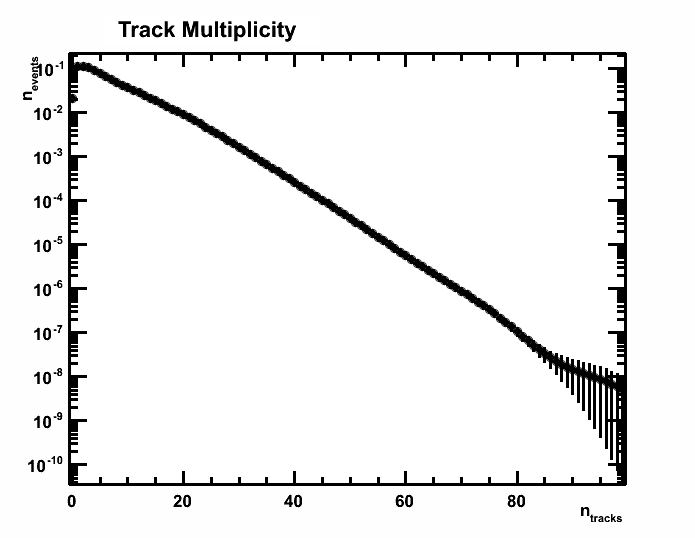
\includegraphics[width=\textwidth]{/afs/cern.ch/user/d/dvoong/cmtuser/DaVinci_v33r6/Phys/ChargedParticleMultiplicity/python/multiplicity/tracks/data_files/TrackMultiplicityPlottingJob/bk/Down/mc/-1/-1/bk/Down/mc/-1/-1/meissner_multiplicity_full/bk/Down/real/-1/-1/bk/Down/real/-1/-1/pngs/background_corrected/2-0_4-5_norm.png}
		\caption{$2.0 \le \eta \le 4.5$}
	\end{subfigure}
	\begin{subfigure}{0.32\textwidth}
		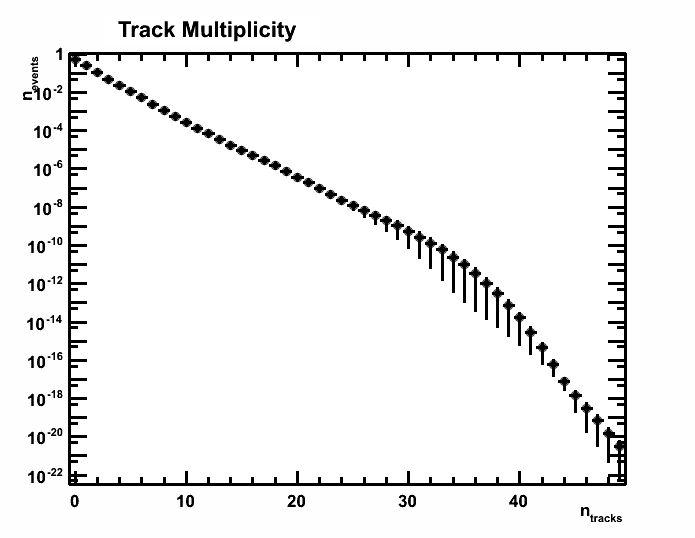
\includegraphics[width=\textwidth]{/afs/cern.ch/user/d/dvoong/cmtuser/DaVinci_v33r6/Phys/ChargedParticleMultiplicity/python/multiplicity/tracks/data_files/TrackMultiplicityPlottingJob/bk/Down/mc/-1/-1/bk/Down/mc/-1/-1/meissner_multiplicity/bk/Down/real/-1/-1/bk/Down/real/-1/-1/pngs/background_corrected/2-0_2-5_norm.png}
		\caption{$2.0 \le \eta \le 2.5$}
	\end{subfigure}
	\begin{subfigure}{0.32\textwidth}
		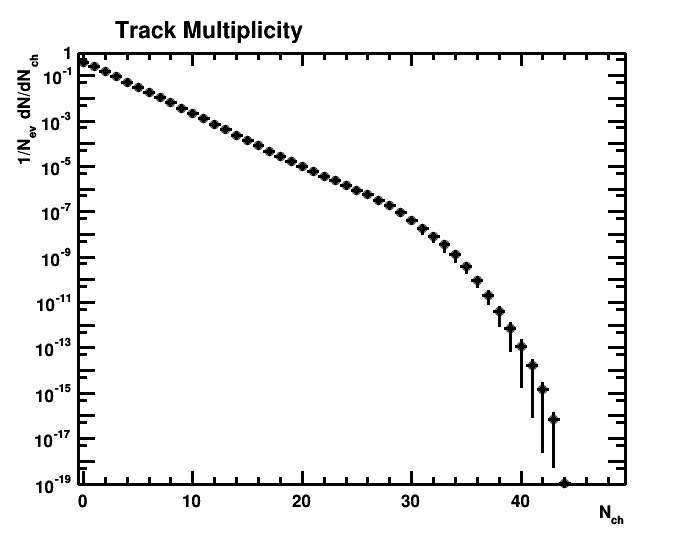
\includegraphics[width=\textwidth]{/afs/cern.ch/user/d/dvoong/cmtuser/DaVinci_v33r6/Phys/ChargedParticleMultiplicity/python/multiplicity/tracks/data_files/TrackMultiplicityPlottingJob/bk/Down/mc/-1/-1/bk/Down/mc/-1/-1/meissner_multiplicity/bk/Down/real/-1/-1/bk/Down/real/-1/-1/pngs/background_corrected/2-5_3-0_norm.png}
		\caption{$2.5 \le \eta \le 3.0$}
	\end{subfigure}
	\begin{subfigure}{0.32\textwidth}
		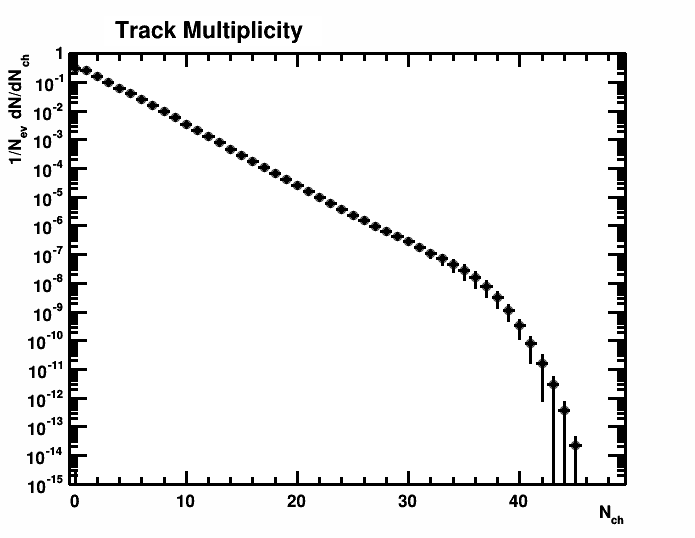
\includegraphics[width=\textwidth]{/afs/cern.ch/user/d/dvoong/cmtuser/DaVinci_v33r6/Phys/ChargedParticleMultiplicity/python/multiplicity/tracks/data_files/TrackMultiplicityPlottingJob/bk/Down/mc/-1/-1/bk/Down/mc/-1/-1/meissner_multiplicity/bk/Down/real/-1/-1/bk/Down/real/-1/-1/pngs/background_corrected/3-0_3-5_norm.png}
		\caption{$3.0 \le \eta \le 3.5$}
	\end{subfigure}
	\begin{subfigure}{0.32\textwidth}
		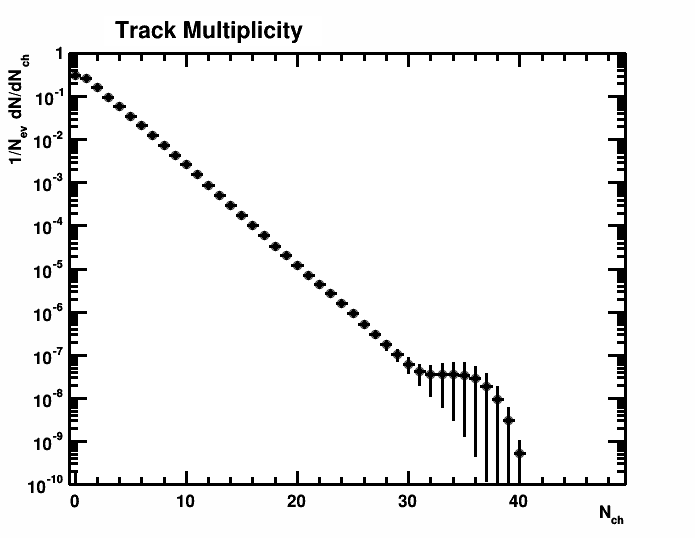
\includegraphics[width=\textwidth]{/afs/cern.ch/user/d/dvoong/cmtuser/DaVinci_v33r6/Phys/ChargedParticleMultiplicity/python/multiplicity/tracks/data_files/TrackMultiplicityPlottingJob/bk/Down/mc/-1/-1/bk/Down/mc/-1/-1/meissner_multiplicity/bk/Down/real/-1/-1/bk/Down/real/-1/-1/pngs/background_corrected/3-5_4-0_norm.png}
		\caption{$3.5 \le \eta \le 4.0$}
	\end{subfigure}
	\begin{subfigure}{0.32\textwidth}
		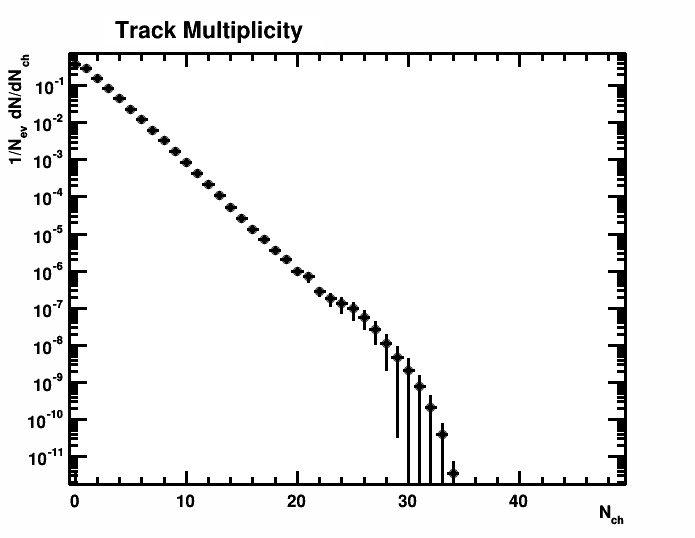
\includegraphics[width=\textwidth]{/afs/cern.ch/user/d/dvoong/cmtuser/DaVinci_v33r6/Phys/ChargedParticleMultiplicity/python/multiplicity/tracks/data_files/TrackMultiplicityPlottingJob/bk/Down/mc/-1/-1/bk/Down/mc/-1/-1/meissner_multiplicity/bk/Down/real/-1/-1/bk/Down/real/-1/-1/pngs/background_corrected/4-0_4-5_norm.png}
		\caption{$4.0 \le \eta \le 4.5$}
	\end{subfigure}
	\caption{Background corrected track multiplicities}
	\label{fig: background corrected track multiplicities}
\end{figure}

\begin{figure}[h]
	\centering
	\begin{subfigure}{0.32\textwidth}
		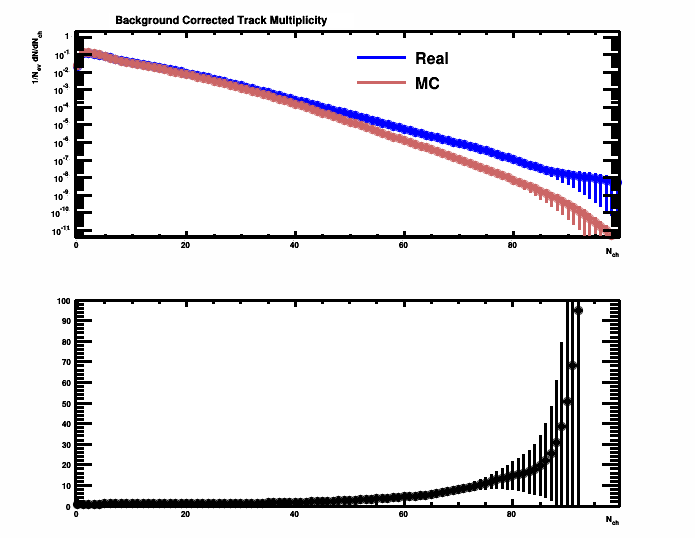
\includegraphics[width=\textwidth]{/afs/cern.ch/user/d/dvoong/cmtuser/DaVinci_v33r6/Phys/ChargedParticleMultiplicity/python/multiplicity/tracks/data_files/TrackMultiplicityPlottingJob/bk/Down/mc/-1/-1/bk/Down/mc/-1/-1/meissner_multiplicity_full/bk/Down/real/-1/-1/bk/Down/real/-1/-1/pngs/comparison/background_corrected/2-0_4-5_comparison.png}
		\caption{$2.0 \le \eta \le 4.5$}
	\end{subfigure}
	\begin{subfigure}{0.32\textwidth}
		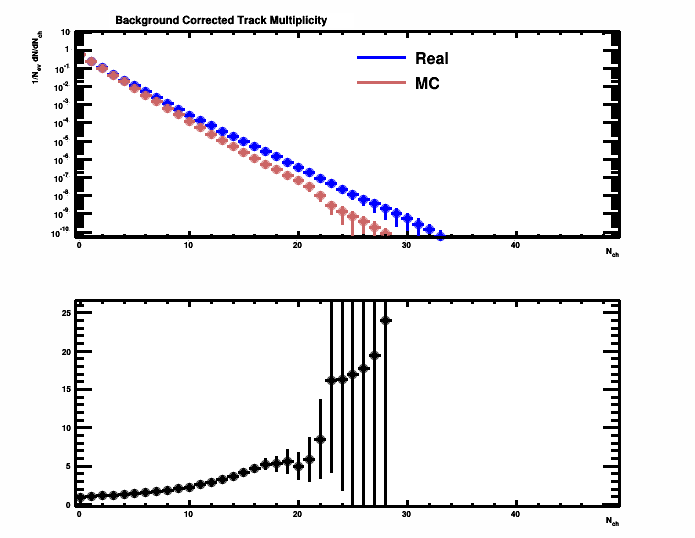
\includegraphics[width=\textwidth]{/afs/cern.ch/user/d/dvoong/cmtuser/DaVinci_v33r6/Phys/ChargedParticleMultiplicity/python/multiplicity/tracks/data_files/TrackMultiplicityPlottingJob/bk/Down/mc/-1/-1/bk/Down/mc/-1/-1/meissner_multiplicity/bk/Down/real/-1/-1/bk/Down/real/-1/-1/pngs/comparison/background_corrected/2-0_2-5_comparison.png}
		\caption{$2.0 \le \eta \le 2.5$}
	\end{subfigure}
	\begin{subfigure}{0.32\textwidth}
		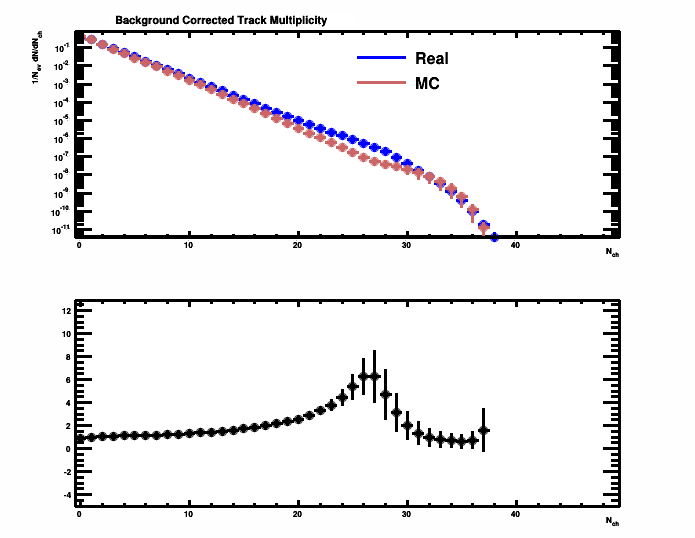
\includegraphics[width=\textwidth]{/afs/cern.ch/user/d/dvoong/cmtuser/DaVinci_v33r6/Phys/ChargedParticleMultiplicity/python/multiplicity/tracks/data_files/TrackMultiplicityPlottingJob/bk/Down/mc/-1/-1/bk/Down/mc/-1/-1/meissner_multiplicity/bk/Down/real/-1/-1/bk/Down/real/-1/-1/pngs/comparison/background_corrected/2-5_3-0_comparison.png}
		\caption{$2.5 \le \eta \le 3.0$}
	\end{subfigure}
	\begin{subfigure}{0.32\textwidth}
		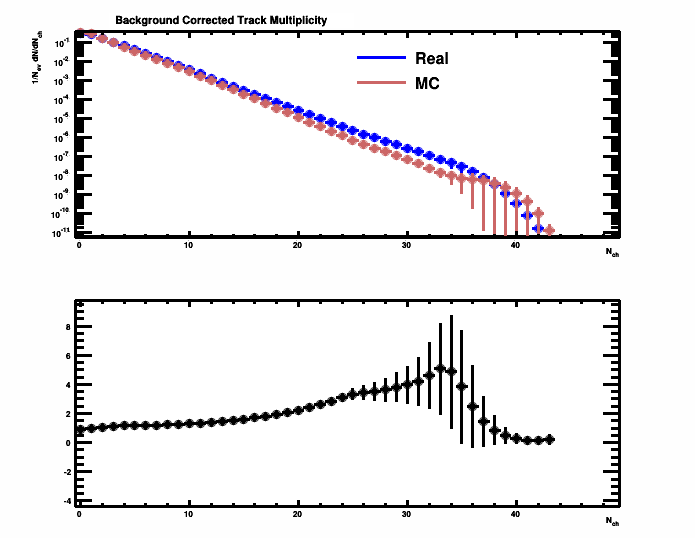
\includegraphics[width=\textwidth]{/afs/cern.ch/user/d/dvoong/cmtuser/DaVinci_v33r6/Phys/ChargedParticleMultiplicity/python/multiplicity/tracks/data_files/TrackMultiplicityPlottingJob/bk/Down/mc/-1/-1/bk/Down/mc/-1/-1/meissner_multiplicity/bk/Down/real/-1/-1/bk/Down/real/-1/-1/pngs/comparison/background_corrected/3-0_3-5_comparison.png}
		\caption{$3.0 \le \eta \le 3.5$}
	\end{subfigure}
	\begin{subfigure}{0.32\textwidth}
		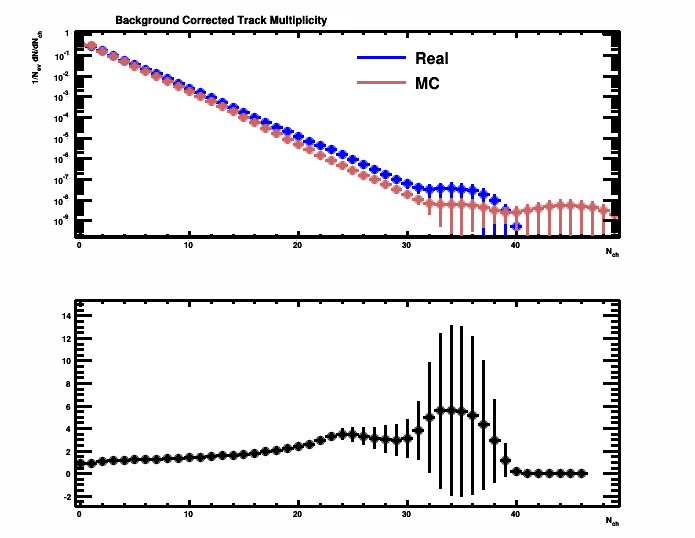
\includegraphics[width=\textwidth]{/afs/cern.ch/user/d/dvoong/cmtuser/DaVinci_v33r6/Phys/ChargedParticleMultiplicity/python/multiplicity/tracks/data_files/TrackMultiplicityPlottingJob/bk/Down/mc/-1/-1/bk/Down/mc/-1/-1/meissner_multiplicity/bk/Down/real/-1/-1/bk/Down/real/-1/-1/pngs/comparison/background_corrected/3-5_4-0_comparison.png}
		\caption{$3.5 \le \eta \le 4.0$}
	\end{subfigure}
	\begin{subfigure}{0.32\textwidth}
		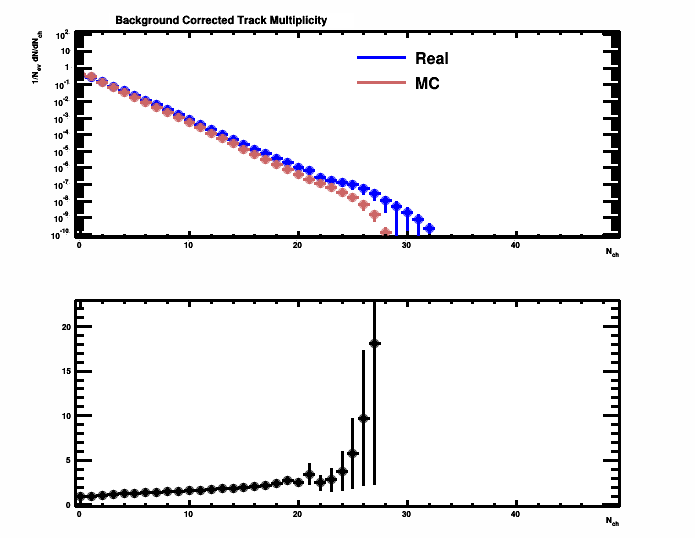
\includegraphics[width=\textwidth]{/afs/cern.ch/user/d/dvoong/cmtuser/DaVinci_v33r6/Phys/ChargedParticleMultiplicity/python/multiplicity/tracks/data_files/TrackMultiplicityPlottingJob/bk/Down/mc/-1/-1/bk/Down/mc/-1/-1/meissner_multiplicity/bk/Down/real/-1/-1/bk/Down/real/-1/-1/pngs/comparison/background_corrected/4-0_4-5_comparison.png}
		\caption{$4.0 \le \eta \le 4.5$}
	\end{subfigure}
	\caption{Background corrected track multiplicities from measured data and MC}
	\label{fig: background corrected track multiplicity comparison}
\end{figure}

\begin{figure}[h]
	\centering
	\begin{subfigure}{0.32\textwidth}
		\includegraphics[width=\textwidth]{/afs/cern.ch/user/d/dvoong/cmtuser/DaVinci_v33r6/Phys/ChargedParticleMultiplicity/python/multiplicity/tracks/data_files/TrackMultiplicityPlottingJob/bk/Down/mc/-1/-1/bk/Down/mc/-1/-1/meissner_multiplicity_full/bk/Down/mc/-1/-1/bk/Down/mc/-1/-1/pngs/cross_check/2-0_4-5.png}
		\caption{$2.0 \le \eta \le 4.5$}
	\end{subfigure}
	\begin{subfigure}{0.32\textwidth}
		\includegraphics[width=\textwidth]{/afs/cern.ch/user/d/dvoong/cmtuser/DaVinci_v33r6/Phys/ChargedParticleMultiplicity/python/multiplicity/tracks/data_files/TrackMultiplicityPlottingJob/bk/Down/mc/-1/-1/bk/Down/mc/-1/-1/meissner_multiplicity/bk/Down/mc/-1/-1/bk/Down/mc/-1/-1/pngs/cross_check/2-0_2-5.png}
		\caption{$2.0 \le \eta \le 2.5$}
	\end{subfigure}
	\begin{subfigure}{0.32\textwidth}
		\includegraphics[width=\textwidth]{/afs/cern.ch/user/d/dvoong/cmtuser/DaVinci_v33r6/Phys/ChargedParticleMultiplicity/python/multiplicity/tracks/data_files/TrackMultiplicityPlottingJob/bk/Down/mc/-1/-1/bk/Down/mc/-1/-1/meissner_multiplicity/bk/Down/mc/-1/-1/bk/Down/mc/-1/-1/pngs/cross_check/2-5_3-0.png}
		\caption{$2.5 \le \eta \le 3.0$}
	\end{subfigure}
	\begin{subfigure}{0.32\textwidth}
		\includegraphics[width=\textwidth]{/afs/cern.ch/user/d/dvoong/cmtuser/DaVinci_v33r6/Phys/ChargedParticleMultiplicity/python/multiplicity/tracks/data_files/TrackMultiplicityPlottingJob/bk/Down/mc/-1/-1/bk/Down/mc/-1/-1/meissner_multiplicity/bk/Down/mc/-1/-1/bk/Down/mc/-1/-1/pngs/cross_check/3-0_3-5.png}
		\caption{$3.0 \le \eta \le 3.5$}
	\end{subfigure}
	\begin{subfigure}{0.32\textwidth}
		\includegraphics[width=\textwidth]{/afs/cern.ch/user/d/dvoong/cmtuser/DaVinci_v33r6/Phys/ChargedParticleMultiplicity/python/multiplicity/tracks/data_files/TrackMultiplicityPlottingJob/bk/Down/mc/-1/-1/bk/Down/mc/-1/-1/meissner_multiplicity/bk/Down/mc/-1/-1/bk/Down/mc/-1/-1/pngs/cross_check/3-5_4-0.png}
		\caption{$3.5 \le \eta \le 4.0$}
	\end{subfigure}
	\begin{subfigure}{0.32\textwidth}
		\includegraphics[width=\textwidth]{/afs/cern.ch/user/d/dvoong/cmtuser/DaVinci_v33r6/Phys/ChargedParticleMultiplicity/python/multiplicity/tracks/data_files/TrackMultiplicityPlottingJob/bk/Down/mc/-1/-1/bk/Down/mc/-1/-1/meissner_multiplicity/bk/Down/mc/-1/-1/bk/Down/mc/-1/-1/pngs/cross_check/4-0_4-5.png}
		\caption{$4.0 \le \eta \le 4.5$}
	\end{subfigure}
	\caption{Background correction cross-check. Background corrected track multiplicities are compared with tracks matched to generator prompt particles by MC truth matching}
	\label{fig: background corrected track multiplicity cross-check}
\end{figure}